\documentclass[12pt]{article}
\usepackage{comment}
\usepackage[left=1in,top=1in,right=1in,bottom=1in]{geometry}
\usepackage[numbers]{natbib}
\usepackage[linktocpage=true]{hyperref}
\usepackage{amsmath, amssymb, amsthm,thmtools}
\usepackage{graphicx}
\usepackage{hyperref}
\usepackage[noabbrev,capitalize]{cleveref}
\usepackage{listings}
\usepackage{enumitem}
\usepackage{titlesec}
\usepackage{setspace} 
\usepackage{mathtools}
\usepackage{xcolor}
\usepackage{tikz}
\usepackage{tikz-cd}
\usepackage[colorinlistoftodos]{todonotes}
\usepackage{algorithm}
\usepackage{algpseudocode}

\setlength{\marginparwidth}{2cm}

\usetikzlibrary{automata,positioning}
\definecolor{crimson}{HTML}{DC143C}

\newcommand{\jv}[1]{\textcolor{red}{\textbf{[JV: } #1\textbf{]}}}
\newcommand{\rt}[1]{\textcolor{red}{\textbf{[RT: } #1\textbf{]}}}

\setlength{\parskip}{6pt}
\setlength{\parindent}{0pt}
\renewcommand{\baselinestretch}{1.2}

\hypersetup{
  colorlinks=true,
  linkcolor=crimson,
  urlcolor=crimson,
  citecolor=crimson
}

\newcounter{foo}
% Theorem Environments
\newtheorem{theorem}{Theorem}
\newtheorem{lemma}[theorem]{Lemma}
\newtheorem{claim}{Claim}
\newtheorem{conjecture}{Conjecture}[foo]
\renewcommand\theconjecture{\Alph{conjecture}}
\newtheorem{definition}[theorem]{Definition}
\newtheorem{corollary}[theorem]{Corollary}
\newtheorem{proposition}[theorem]{Proposition}
\newtheorem{oldtheorem}[foo]{Theorem}
\renewcommand\theoldtheorem{\Alph{oldtheorem}}

\newcommand{\Var}{\mathrm{Var}} 
\newcommand{\Cov}{\mathrm{Cov}} 
\newcommand{\Bias}{\mathrm{Bias}} 
\newcommand*{\Z}{\mathbb{Z}} 
\newcommand*{\Q}{\mathbb{Q}} 
\newcommand*{\R}{\mathbb{R}} 
\newcommand*{\C}{\mathbb{C}} 
\newcommand*{\N}{\mathbb{N}} 
\newcommand*{\prob}{\mathds{P}} 
\newcommand*{\E}{\mathds{E}} 
\newcommand*{\F}{\mathcal{F}}
\newcommand*{\ex}{\textnormal{ex}}
\newcommand*{\con}{\mathcal{C}}

% Title Page
\title{Double Turán Problem}
\author{Ray Tsai \\ Advisor: Prof. Jacques Verstraete}

\begin{document}

\maketitle

% \begin{abstract} Your abstract here. Provide a concise summary of your thesis, including the problem statement, methodology, main results, and conclusions. \end{abstract}

% \section*{Acknowledgments} Thank your advisor, collaborators, and anyone who supported your research.

\vspace*{-1cm}

\tableofcontents

\newpage

\section{Introduction}

This thesis focuses on a variation of the \textit{Turán problem} in extremal combinatorics.  The fundamental question in extremal hypergraph theory is determining the maximum number of edges in an $n$-vertex $r$-uniform graph that does not contain a prescribed $r$-uniform graph $F$ as a subgraph. These maxima, denoted $\ex(n, F)$, are referred to as the \textit{extremal numbers} or \textit{Turán numbers} for $F$. One of the cornerstones of extremal graph theory, concerning the case $F$ is a clique, is Tur\'{a}n's Theorem~\cite{Turan1941}. To state the theorem, we need the \textit{Tur\'{a}n graphs} $T_k(n)$, which denotes a complete multipartite graph with $n$ vertices and $k$ parts of size $\lfloor n/k\rfloor$ or $\lceil n/k\rceil$. 

\begin{oldtheorem}[Tur\'{a}n's Theorem]\label{thm:turan}
The maximum number of edges in an $n$-vertex graph containing no clique of order $r + 1$ is $e(T_r(n))$, with equality only for $T_r(n)$.
\end{oldtheorem}

Simonovits~\cite{ErdosSimonovits1966} observed via the Erd\H{o}s-Stone Theorem~\cite{ErdosStone1946} that the asymptotic value of $\ex(n, F)$ may be obtained whenever $F$ is non-bipartite:

\begin{oldtheorem}[Erd\H{o}s-Stone Theorem, Simonovits' Theorem]\label{thm:ess}
Let $F$ be any graph of chromatic number $r + 1 \geq 3$. Then $\ex(n, F) = (1 + o(1))T_r(n)$ as $n \rightarrow \infty$.
\end{oldtheorem}

There are a number of proofs of the Erd\H{o}s-Stone Theorem. A very general framework involves \textit{Szemer\'{e}di's Regularity Lemma}, which may be stated as follows. A pair $(U,V)$ of disjoint sets of vertices in a graph $G$ is called \textit{$\epsilon$-regular} if for any $X \subseteq U$ and $Y \subseteq V$ of size at least $\epsilon |U|$ and $\epsilon|V|$ respectively, 
\[
  \left|\frac{e(X, Y)}{|X||Y|} - \frac{e(U, V)}{|U||V|}\right| < \epsilon.
\]
The following was proved by Szemer\'{e}di~\cite{Szemeredi1978}:

\begin{oldtheorem} [Szemer\'{e}di's Regularity Lemma]
For all $\epsilon > 0$, there exist $m$ and $M$ such that for every graph $G$, there exists a partition $(V_1, V_2, \dots, V_k)$ of $V(G)$ such that $m \leq k \leq M$ and $|V_1| \leq |V_2| \leq \dots \leq |V_k| \leq |V_1| + 1$ and all but at most $\epsilon k^2$ pairs $(V_i, V_j)$ are $\epsilon$-regular. 
\end{oldtheorem}

The value of $\ex(n, F)$ for bipartite $F$ is in general wide open, and the order of magnitude of $\ex(n, K_{4, 4})$ or $\ex(n, C_8)$ is not known -- see F\"{u}redi and Simonovits~\cite{FurediSimonovits2013} for a history of the bipartite Tur\'{a}n problem. There is also no analog of the above theorems for $r$-uniform hypergraphs; the asymptotic value of $\ex(n, K_k^r)$ is not known for any $k > r \geq 3$, where $K_k^r$ denotes the complete $r$-uniform hypergraph on $k$ vertices. The asymptotic value of $\ex(n, K_4^3)$ was conjectured by Tur\'{a}n~\cite{Turan1941} to be $\frac{5}{9} \binom{n}{3}$, and this remains open despite decades of intensive research. 

In this thesis, we investigate closely related problems which we refer to as \textit{double Tur\'{a}n problems}. To describe these problems, let $G_1, G_2, \ldots, G_m$ be graphs with the same vertex set $V(G_i) = [n]$ for $i \in [m]$. For a graph $F$, we say that $G_1, G_2, \dots, G_m$ is \textit{double $F$-free} if $E(F) \not \subseteq E(G_i) \cap E(G_j)$ for $1 \leq i < j \leq m$. In other words, $F$ does not appear in the intersection of any two of the graphs $G_i$. We call a copy of $F$ in the intersection of two of the graphs $G_i$ a \textit{double $F$}. Let $\phi(m, n, F)$ denote the maximum value of $\sum_{i = 1}^m e(G_i)$ such that $G_1, G_2, \dots, G_m$ does not contain a double $F$. We say that graphs $G_1, G_2, \dots, G_m$ are \textit{induced} to mean that every $G_i$ is an induced subgraph of $\bigcup_{i = 1}^m G_i$. In other words, if $\{u,v\} \in E(G_i)$ and $u,v \in V(G_j)$, then $\{u,v\} \in E(G_j)$. Let $\phi^*(m, n, F)$ denote the maximum value of $\sum_{i = 1}^m e(G_i)$ such that $G_1, G_2, \dots, G_m$ does not contain a double $F$ and $G_1, G_2,\dots, G_m$ are induced. Clearly, $\phi^*(m, n, F) \leq \phi(m, n, F)$, and the study of $\phi^*(m, n, F)$ and $\phi(m, n,F )$ is motivated by certain hypergraph extremal problems.

\subsection{Link graphs and hypergraphs}

Apart from the intrinsic interest in studying $\phi(m, n, F)$, a motivation is that $\phi(m, n, F)$ is closely connected to pure hypergraph extremal problems via the notion of \textit{link graphs}. Let $H$ be a triple system, that is, a set of three-element subsets of a finite set $[n]$. These three-element subsets form the edge-set $E(H)$ of $H$, while $V(H) = V$ is the vertex set of $H$. For $i \in V(H)$, the \textit{link graph} of $i$,  denoted $H_i$, is the graph with $V(H_i) = V(H) \backslash \{i\}$ and $E(H_i) = \{\{j, k\} : \{i, j, k\} \in E(H)\}$. A handy idea in extremal hypergraph theory is to reduce a hypergraph extremal problem to extremal problems for the link graphs. For instance, a triple system $H$ does not contain a tetrahedron, i.e. four triples on four vertices, if and only if all its link graphs are triangle-free.

In the current context, given a graph $F$, let $F^+$ denote the triple system with $V(F^+) = V(F) \cup \{x, y\}$ and $E(F^+) = \{e \cup \{x\}, e \cup \{y\} : e \in E(F)\}$. Then $\phi(n, n, F)$ and $\ex(n, F^+)$ are intimately related: if $H$ is an $F^+$-free triple system with vertex set $[n]$, then clearly the link graphs $H_1, H_2, \dots, H_n$ are double $F$-free, which implies $\ex(n, F^+) \leq \phi(n, n, F)$. This relates the double Tur\'{a}n problem to hypergraph extremal problems.

Now let $G$ be the graph consisting of all pairs contained in triples in $F^+$. The \textit{generalized Tur\'{a}n problem} asks for the maximum number $\ex(n, G, K_3)$ of triangles in a graph $H$ with vertex set $[n]$ that does not contain $G$. This problem was studied by Alon and Shikhelman~\cite{AlonShikhelman2016} and Kostochka, Mubayi and Verstraete~\cite{KostochkaMubayiV2015,MubayiMukherjee2023,MubayiV2016}. Similar to how link graphs relate to hypergraph extremal problems, the generalized Tur\'{a}n problem is related to $\phi^*(n, n, F)$ as follows: define $H_i = \{\{j, k\} : \{i, j\}, \{j, k\}, \{i, k\} \in E(H)\}$. Then $H_1, H_2, \dots, H_n$ are induced and double $F$-free, so $\phi^*(n, n, F) \geq \ex(n, G, K_3)$. This relates the induced double Tur\'{a}n problem to extremal problems for triangles in graphs.

\subsection{Main results : the induced case}

The determination of $\phi^*(m, n, F)$ turns out to be fairly straightforward when $F$ is a non-bipartite graph: the extremal objects are simply $m$ copies of the same extremal graph for $F$.

\begin{theorem}\label{thm:inducedF}
  For $r \geq 3$, there exists $n_0(r)$ such that if $n \geq n_0(r)$ and $F$ is a graph of chromatic number $r$, then for all $m \geq 3$,    
  \[
    \phi^*(m, n, F) = m \cdot \ex(n, F),
  \]
  with equality only for identical extremal $n$-vertex $F$-free graphs.
\end{theorem}

In the case $F = K_r$, we shall see the theorem is true for all $n \geq 3$:

\begin{theorem}\label{thm:complete}
Let $m, n, r \geq 3$. Then $\phi^*(m, n, K_{r}) = m \cdot e(T_{r - 1}(n))$ with equality for induced $K_{r}$-free graphs $G_1, G_2, \dots, G_m$ only if $G_1 = G_2 = \dots = G_m = T_{r - 1}(n)$.  
\end{theorem}

In the case $F$ is a bipartite graph, even determining the order of magnitude of $\phi^*(m, n, F)$ appears to be difficult. In fact, we do not even know the order of magnitude of $\phi^*(m, n, P)$ when $P$ is a path with two edges. In this thesis, we propose the following very broad conjecture:

\begin{conjecture}\label{conj:main}
Let $F$ be any non-empty graph and $m, n \geq 1$. Then 
\[ 
  \phi^*(m, n, F) = \Theta(m \cdot \ex(n, F) + n^2).
\]
\end{conjecture}

It is clear that a single complete graph $K_n$ does not contain a double $F$, and neither do identical copies $G_1, G_2, \dots, G_m$ of an extremal $n$-vertex $F$-free graph. Thus we have the trivial lower bound 
\[ 
  \phi^*(m, n, F) \geq \max\left\{\binom{n}{2}, m \cdot \ex(n, F)\right\}.
\]

This conjecture is true when $F$ is non-bipartite, by Theorem \ref{thm:inducedF}. If $F$ is bipartite, then the upper bounds on $\phi^*(m, n, F)$ are more difficult to come by, especially when $m$ is large. For instance, we know 
\[ 
  \ex(n, K_{2,2,2}, K_3) \leq \phi^*(n, n, K_{2,2}),
\]
and so Conjecture \ref{conj:main} implies that an $n$-vertex graph not containing the octahedron graph has $O(n^{5/2})$ triangles. In fact, it is also the case that $\ex(2n, K_{2,2,2}, K_3) \geq \phi^*(n, n, K_{2,2})$: if we have double $K_{2,2}$-free induced graphs $G_1, G_2, \dots, G_{n}$ with vertex set $[n]$, then let $H$ be the graph with $V(H) = [2n]$ consisting of all triangles with vertex set $\{i, j, k\}$ such that $n < k \leq 2n$ and $\{i, j\} \in E(G_k)$. The graph $H$ is $K_{2, 2, 2}$-free and $|E(H)| = \sum_{i = 1}^{n/2} e(G_i)$. Similarly, we have
\[ 
  \ex(n, K_{1, 2, 2}, K_3) \leq \phi^*(n, n, K_{1,2})
\]
and so Conjecture \ref{conj:main} implies that an $n$-vertex graph not containing the wheel graph has $O(n^{2})$ triangles, which is conjectured by Mubayi and Verstraete~\cite{MubayiV2016}. The conjecture proposes more generally that if $F$ is a tree, then $\phi^*(n, n, F) = O(n^2)$. In fact, it is possible to prove the following theorem using the \textit{removal lemma} as in~\cite{MubayiMukherjee2023} as well as a construction for $\phi(n, n, P)$ in this work:

\begin{theorem}\label{thm:inducedP}
Let $P$ be a path with two edges. Then $\phi(n, n, P) = \Omega(n^{5/2})$, whereas $\phi^*(n, n, P) = o(n^{5/2})$, as $n \rightarrow \infty$. In particular, 
\[ 
  \lim_{n \rightarrow \infty} \frac{\phi^*(n, n, P)}{\phi(n, n, P)} = 0.
\]
\end{theorem}

If $M$ is a matching with two edges, and $M^+$ is the graph obtained from two copies of $K_4$ sharing one edge by removing that edge, then $\ex(n, M^+, K_3) \leq \phi^*(n, n, M)$. If $F$ is the triple system consisting of all four triangles in $M^+$, then F\"{u}redi~\cite{Furedi1984} showed $\ex(n, M^+) = O(n^2)$, answering a conjecture of Erd\H{o}s~\cite{Erdos1977}. It is possible to adapt F\"{u}redi's proof to give $\phi^*(n, n, M) = O(n^2)$, so in this case, $\ex(n, M^+, K_3) = \Theta(\phi^*(n, n, M))$. For improvements of the constant factor, see Mubayi and Verstraete~\cite{MubayiV2004} and Pikhurko and Verstraete~\cite{PikhurkoV2009}. We shall see that for some bipartite $F$, if $m$ is not too large relative to $n$, then Conjecture \ref{conj:main} is also true. 

\subsection{Main results : the non-induced case}

Determining $\phi(m, n, F)$ even when $F$ is a complete graph is challenging. The forth theorem we give is well-suited to the case of certain bipartite graphs, and is due to Wilson:

\begin{theorem}\label{wilsontheorem}
  Let $F$ be a graph. If there exists an extremal $F$-free $n$-vertex graph with maximum degree at most $n^{1/2}/m^2$, then 
  \[ 
    \phi(m, n, F) = \binom{n}{2} + \binom{m}{2}\ex(n,F).
  \]
\end{theorem}

Since $\binom{n}{2} + m - 1 \leq \phi^*(m, n, F) \leq \phi(m, n, F)$ for any graph $F$ with at least two edges, this theorem shows $\phi^*(m, n, F) = (1 + o(1))\binom{n}{2}$ whenever the conditions on $m$ in the theorem are satisfied. In particular, if $P$ is the path with two edges, and $m = o(n^{1/4})$ as $n \rightarrow \infty$, then 
\[ 
  \binom{n}{2} + m - 1 \leq \phi^*(m, n, P) \leq \phi(m, n, P) = \binom{n}{2} + \binom{m}{2} \left\lfloor \frac{n}{2}\right\rfloor. 
\]
When $F$ is bipartite, the value of $\phi(m, n, F)$ for larger $m$ appears to be difficult to determine. We investigate the case $F = P$ more closely. 

\begin{theorem}\label{thm:pm}
Let $P$ be the path with two edges. Then as $n \rightarrow \infty$,
\[
  \phi(m, n, P) = \begin{cases}
    \left(\frac{1}{2} + o(1)\right)n^2, & \sqrt{n}/m \to \infty \\
    \Theta(n^2), & m = \Theta(\sqrt{n}) \\
    \left(\frac{1}{2} + o(1)\right)mn^{3/2}, & \sqrt{n} < m \leq n \\
    \left(\frac{1}{2} + o(1)\right)\sqrt{m}n^{2}, & n < m \leq n^2 \\
    \Theta(n^3), & m = \Theta(n^2) \\
    \left(1 + o(1)\right)mn, & m/n^2 \to \infty
  \end{cases}
\]
\end{theorem}

Interestingly, while Conjecture \ref{conj:main} proposes $\phi^*(m, n, P) = O(n^2 + mn)$ for all $m,n \geq 1$, the above theorem shows $\phi(m, n, P)$ is much larger, of order at least $mn^{3/2}$ when $m \geq \sqrt{n}$.  

Our first theorem on $\phi(m, n, F)$ for non-bipartite graphs $F$ uses the notion of \textit{supersaturation} -- see Erd\H{o}s and Simonovits~\cite{ErdosSimonovits1983}. We determine the asymptotic value of $\phi(m, n, F)$ as $m \rightarrow \infty$ when $F$ is a non-bipartite graph:

\begin{theorem}\label{thm:asymp}
  Let $n \geq 1$ and let $F$ be a non-bipartite graph. Then as $m \rightarrow \infty$, 
  \[
    \phi(m, n, F) = (1 + o(1))m \cdot \ex(n, F).
  \]
\end{theorem}

The next result we present concerns non-bipartite graphs. To state the theorem, we require the notion of $M$-color Ramsey numbers. Define $R_M(r)$ to be the \textit{$M$-color Ramsey number} for the complete graph $K_r$, that is, the minimum $N$ such that there exists a monochromatic $F$ in any coloring of $E(K_N)$ with $M$ colors. Suppose we have a monochromatic $K_r$-free coloring $c : E(K_N) \rightarrow 2^{[m]}$. For $i \in [m]$, let $H_i = \{\{u, w\} \in E(K_N) : i \in c(u, w)\}$. Then $H_1,H_2,\dots,H_m$ are double $K_r$-free. If we replace the vertices of $K_N$ with disjoint sets $V_1, V_2, \ldots, V_N$ whose sizes add up to $n$, and then let
\[ 
  G_i = \{\{x,y\} : (x,y) \in V_u \times V_w, \, i \in c(u, w), \, 1 \leq u < w \leq N\}
\] 
and make each $V_i$ cliques in $G_1$, then $G_1, G_2, \dots, G_m$ is also double $K_r$-free. We call $G_1, G_2, \dots, G_m$ an $(m, n, N)$-blowup. 

\begin{center}
  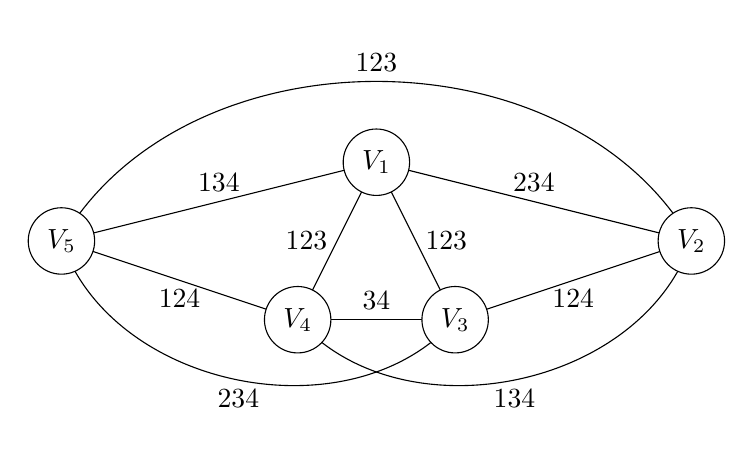
\begin{tikzpicture}
    \draw[bend right=60] (4, 0.5) to node[midway, above] {$123$} (-4, 0.5); 
    \draw (-4, 0.5) to node[midway, below] {$124$} (-1, -0.5); 
    \draw (-1, -0.5) to node[midway, above] {$34$} (1, -0.5); 
    \draw (1, -0.5) to node[midway, below] {$124$} (4, 0.5); 
    \draw (0, 1.5) to node[midway, above] {$234$} (4, 0.5); 
    \draw (0, 1.5) to node[midway, above] {$134$} (-4, 0.5); 
    \draw (0, 1.5) to node[midway, left] {$123$} (-1, -0.5); 
    \draw (0, 1.5) to node[midway, right] {$123$} (1, -0.5); 
    \draw[bend left=60] (4, 0.5) to node[midway, below] {$134$} (-1, -0.5); 
    \draw[bend right=60] (-4, 0.5) to node[midway, below] {$234$} (1, -0.5);

    \foreach [count=\i] \x/\y in {0/1.5, 4/0.5, 1/-0.5, -1/-0.5, -4/0.5} { 
      \fill[white] (\x, \y) circle (12pt);
      \draw (\x, \y) circle (12pt);
      \node at (\x, \y) [] {$V_{\i}$}; 
    }
  \end{tikzpicture}
  \\
  \small{Example of an $(4, n, 5)$-blowup not containing a double $K_3$.}
\end{center}

Let $f(m, n, r)$ denote the maximum of $e(G_1) + e(G_2) + \dots + e(G_m)$ such that $G_1, G_2, \dots, G_m$ is a double $K_r$-free $(m, n, N)$-blowup for some $N < R_{\binom{m}{2}}(r)$. This turns out to be exactly the construction which determines $\phi(m, n, F)$ when $F$ is a complete graph: 

\begin{theorem}\label{thm:blowup}
Let $r \geq 2$ and $m,n \geq 1$. Then 
\[ 
  \phi(m, n, K_r) = f(m, n, r).
\]
\end{theorem}

While computing $f(m, n, r)$ is a finite calculation, the Ramsey number $R_{\binom{m}{2}}(r)$ unfortunately appears to be intractable in general; it is known that $R_2(3) = 6$ and $R_3(3) = 17$ and $R_2(4) = 18$, but no further multicolor Ramsey numbers are known~\cite{ConlonFerber2021,Lefmann1987}. In the special case $r = m = 3$, the following holds: 

\begin{theorem}\label{thm:triangles}
  For all $n \geq 1$,
  \[
    \phi(3, n, K_3) = \binom{n}{2} + \left\lfloor \frac{n^2}{2} \right\rfloor.
  \]
\end{theorem}

\subsection{Definitions and Notations}

Denote the set of first $n$ positive integers as $[n] = \{1, 2, \ldots, n\}$. Given a set $X$, we denote $2^X$ as the power set of $X$. Let $G = (V, E)$ be a graph. Let $V(G)$ denote the vertex set and $E(G)$ denote the edge set of $G$. Let $e(G) = |E(G)|$ be the number of edges in $G$. For vertex $v \in V(G)$, we denote by $N_G(v) = \{u \in V(G) : \{u, v\} \in E(G)\}$ the neighborhood of $v$. Given two graphs $G_1, G_2$, we denote $G_1 \cup G_2$ as the graph on $V(G_1) \cup V(G_2)$ with edge set $E(G_1 \cap G_2) = E(G_1) \cup E(G_2)$. Similarly, we define $G_1 \cap G_2$ as the graph on $V(G_1) \cap V(G_2)$ with edge set $E(G_1 \cap G_2) = E(G_1) \cap E(G_2)$. In this thesis, we reserve $n$ to denote the number of vertices in a graph. We call a $n$-vertex complete graph $K_n$, and a complete bipartite graph $K_{a, b}$, where $a, b$ are the sizes of its parts. Given graph $G, H$, define $G + H$ as the graph fully connecting $G, H$, i.e. $V(G + H) = V(G) \cup V(H)$ and $E(G + H) = E(G) \cup E(H) \cup \{\{u, v\} : u \in V(G), v \in V(H)\}$. Given graphs $G$ and $F$, we say that $G$ is $F$-free if $G$ does not contain $F$ as a subgraph. We denote $\ex(n, F)$ to be the maximum possible number of edges an $F$-free graph on $n$ vertices, and we call a $F$-free graph achieving this maximum an extremal graph for $F$. Let $v$ be a vertex from $G_1, G_2, \ldots, G_m$. Unless otherwise specified, we denote $d(v)$ as the sum of the degree of $v$ over all $G_i$.

\section{The induced double Tur\'{a}n problem}

We prove the theorems for $\phi^*(m, n ,F)$ in this chapter. In particular, the main theorem we prove is Theorem \ref{thm:inducedF} for general non-bipartite graphs $F$ and in the special case of cliques. We will first introduce two observations that significantly simplify the problem.

The first observation is that the determination of $\phi^*(m, n, F)$ can be reduced down to the case of two graphs, which is stated in the following lemma:

\begin{lemma}\label{lem:induce-reduce}
  Let $n, m, k \geq 2$ with $m \geq k$, $F$ be some graph. Then
  \[
    \phi^*(m, n, F) \leq \frac{m}{k} \cdot \phi^*(k, n, F).
  \]
  Moreover, let $G_1, \ldots, G_m$ be induced double $F$-free graphs on $[n]$ and suppose $\sum_{i = 1}^k e(G_i) = \phi^*(k, n, F)$ only if $G_1 = \cdots = G_k$. Then $\sum_{i = 1}^m e(G_i) = \phi^*(m, n, F)$ only if $G_1 = \cdots = G_m$.
\end{lemma}

\begin{proof}
  Let $G_1, \ldots, G_m$ be induced double $F$-free graphs on $[n]$. Put $G_{i + m} = G_i$ for all $i \in [m]$. Then
  \[
    \sum_{i = 1}^m e(G_i) = \frac{1}{k}\sum_{i = 1}^m [e(G_i) + \cdots + e(G_{i + k - 1})] \leq \frac{1}{k}\sum_{i = 1}^m \phi^*(k, n, F) = \frac{m}{k} \cdot \phi^*(k, n, F),
  \]
  which establishes the upper bound. The lower bound follows from the construction with $G_1 = \cdots = G_m$ to be $n$-vertex extremal graphs for $F$.

  Now suppose $\sum_{i = 1}^m e(G_i) = (m/k)\phi^*(k, n, F)$ and $G_1 \neq G_2$. By assumption $\sum_{i = 1}^k e(G_i) < \phi^*(k, n, F)$. But then $\sum_{i = 1}^k e(G_{i + j}) > \phi^*(k, n, F)$ for some $j \geq 1$, contradiction. 
\end{proof}

Now that we may determine $\phi^*(m, n, F)$ by examining $\phi^*(m, n, F)$, the second observation is that $\phi^*(m, n, F)$ can be further reduced to a finite optimization problem on a single variable. To state the lemma, we introduce the following construction function: 

\begin{definition}
  For $n \geq t \geq 1$ and $F$ some graph, define 
  \[
    \con(n, t, F) \coloneq \binom{n - t}{2} + (n - t)t + 2\ex(t, F).
  \]
  The construction described by $\con(n, t, F)$ are graphs $G_1, G_2$ on $[n]$, such that $G_2$ is a $t$-vertex extremal graph for $F$ and $G_1 = G_2 + K_{n - t}$. 
\end{definition}

\begin{lemma}\label{lem:optimize-con}
  Let $F$ be some graph. For $n \geq 1$,
  \[
    \phi^*(2, n, F) = \max_{0 \leq t \leq n} \con(n, t, F).
  \]
  Moreover, the equality holds for graphs $G_1, G_2$ on $[n]$ only if $G_1, G_2$ are the construction described by $\con(n, t_{max}, F)$, where $t_{max} \in [n]$ is a maximizer for $\con(n, t, F)$.
\end{lemma}

\begin{proof}
  Let $G_1, G_2$ be induced double $F$-free graphs on $[n]$. Put $T = V(G_1) \cap V(G_2)$, $t = |T|$, $s = |V(G_1) \backslash T|$, and $n - t - s = |V(G_2) \backslash T|$. Note that $t, s \in \Z_{\geq 0}$. Since $G_1, G_2$ are induced subgraphs of $G_1 \cup G_2$, we have $G_1[T] = G_2[T] = G_1 \cap G_2$. But then $G_1 \cap G_2$ is $F$-free, so $e(G_1[T]) = e(G_2[T]) \leq \ex(t, F)$. Notice there can be at most $t(n - t)$ edges between $T$ and $(V(G_1) \cup V(G_2)) \backslash T$. Since $G[V(G_1) \backslash T] \leq \binom{s}{2}$ and $G[V(G_2) \backslash T] \leq \binom{n - t - s}{2}$,
  \[
    e(G_1) + e(G_2) \leq \binom{s}{2} + \binom{n - s - t}{2} + t(n - t) + 2\ex(t, F).
  \]
  But then $\binom{n - t}{2} > \binom{s}{2} + \binom{n - t - s}{2}$ for $0 < s < n - t$, so
  \[
    e(G_1) + e(G_2) \leq \binom{n - t}{2} + (n - t)t + 2\ex(t, F) = \con(n, t, F).
  \]
  This establishes the upper bound. From this we also know that $e(G_1) + e(G_2) = \con(n, t, F)$ only if $G_1, G_2$ are the construction described by $\con(n, t, F)$. The result now follows.
\end{proof}

\subsection{Proof of Theorem \ref{thm:complete}}

By \cref{lem:induce-reduce}, it suffices to prove the theorem for $m = 3$. Let $G_1, G_2, G_3$ be induced double $K_r$-free graphs, such that $e(G_1) + e(G_2) + e(G_3) = \phi^*(3, n, K_r)$. We may assume $e(G_1) \geq e(G_2) \geq e(G_3)$, and we already know $\phi^*(3, n, K_r) \geq 3\ex(n, K_r)$. Consequently, we must have $e(G_1) + e(G_2) \geq 2\ex(n, K_r)$. Since $G_1, G_2, G_3$ are induced and $e(G_1) + e(G_2) + e(G_3) \geq 3\ex(n, K_r)$, it suffices to show that $G_1 = G_2 = T_{r - 1}(n)$. In particular, we will use \cref{lem:optimize-con} to show that $G_1, G_2$ is an extremal configuration without containing a double $K_r$. 

Let $t = |V(G_1 \cap G_2)|$. By Turán's Theorem,
\[
  \ex(t, K_{r}) - \ex(t - 1, K_{r}) = e(T_{r - 1}(t)) - e(T_{r - 1}(t - 1)) = t - \left\lceil \frac{t}{r - 1} \right\rceil.
\]
It immediately follows that
\begin{equation}
  \con(n, t, K_r) - \con(n, t - 1, K_r) = - t + 1 + 2[\ex(t, K_r) - \ex(t - 1, K_r)] = t + 1 - 2\left\lceil \frac{t}{r - 1} \right\rceil. \label{eq:con1}
\end{equation}
For $r \geq 4$, $\con(n, t, K_r)$ is strictly increasing on $t$, so by \cref{lem:optimize-con}, 
\[
  \phi^*(2, n, K_r) = \con(n, n, K_r) = 2\ex(n, K_r) = e(G_1) + e(G_2)
\]
and $G_1 = G_2 = T_{r - 1}(n)$, as desired. 

Now suppose $r = 3$. Equation \eqref{eq:con1} shows that $\con(n, t, K_r)$ is non-decreasing on $t$ and $\con(n, t, K_r) > \con(n, t, K_r)$ for even $t$. By \cref{lem:optimize-con}, we now have 
\[
  \phi^*(2, n, K_r) = \max[\con(n, n, K_r), \con(n, n - 1, K_r)] = 2\ex(n, K_r) = e(G_1) + e(G_2),
\]
and either $G_1 = G_2 = T_{r - 1}(n)$, or $G_2 = T_{r - 1}(n - 1)$ and $G_1 = G_2 + K_1$. If the latter case is true, then $e(G_3) \geq \ex(n, F) > e(G_2)$, and this contradiction completes the proof. \qed

\subsection{Proof of Theorem \ref{thm:inducedF}}

If $F$ is a graph of chromatic number $r + 1 \geq 3$, then Theorem \ref{thm:ess} shows 
$\ex(n,F)= (1 + o(1))\ex(n,K_{r+1})$ as $n \rightarrow \infty$. In this section, we prove Theorem \ref{thm:inducedF} following the same line of reasoning as in the proof of Theorem \ref{thm:complete}.

\begin{proof}[Proof of Theorem \ref{thm:inducedF}]
  By \cref{lem:induce-reduce}, it suffices to prove the theorem for $m = 3$. Let $G_1, G_2, G_3$ be induced double $F$-free graphs, such that $e(G_1) + e(G_2) + e(G_3) = \phi^*(3, n, F)$. We may assume $e(G_1) \geq e(G_2) \geq e(G_3)$, and we already know $\phi^*(3, n, F) \geq 3\ex(n, F)$. Consequently, we must have $e(G_1) + e(G_2) \geq 2\ex(n, F)$. Since $G_1, G_2, G_3$ are induced and $e(G_1) + e(G_2) + e(G_3) \geq 3\ex(n, F)$, it suffices to show that $G_1 = G_2$ are $n$-vertex $F$-free extremal graphs. In particular, we will use \cref{lem:optimize-con} to show that $G_1, G_2$ is an extremal configuration without containing a double $F$.
  
  Let $t = |V(G_1 \cap G_2)|$. If $t < \sqrt{n}$, then
  \[
    2\ex(n, F) \geq 2e(T_{r - 1}(n)) \geq 2\left\lfloor\frac{n^2}{4}\right\rfloor \geq \binom{n}{2} + \binom{\sqrt{n}}{2} > \con(n, t, F).
  \]
  Thus $t \geq \sqrt{n}$. But then for large enough $t$, any extremal $t$-vertex $F$-free graph contains a spanning complete $(r - 1)$-partite subgraph $T_{r - 1}(t)$, so we may add $\ex(t - 1, F) - e(T_{r - 1}(t - 1))$ egdes to $T_{r - 1}(t)$ and still avoid $F$ as a subgraph. Hence for large enough $t$, we have $\ex(t, F) \geq \ex(t - 1, F) - e(T_{r - 1}(t - 1)) + e(T_{r - 1}(t))$, and so
  \[
    \ex(t, F) - \ex(t - 1, F) \geq e(T_{r - 1}(t)) - e(T_{r - 1}(t - 1)) \geq t - \left\lceil \frac{t}{r - 1} \right\rceil.
  \]
  It immediately follows that
  \begin{equation}
    \con(n, t, F) - \con(n, t - 1, F) = - t + 1 + 2[\ex(t, F) - \ex(t - 1, F)] \geq t + 1 - 2\left\lceil \frac{t}{r - 1} \right\rceil. \label{eq:con}
  \end{equation}
  For $r \geq 4$, $\con(n, t, F)$ is strictly increasing on $t$, so by \cref{lem:optimize-con}, 
  \[
    \phi^*(2, n, F) = \con(n, n, F) = 2\ex(n, F) = e(G_1) + e(G_2),
  \] 
  and $G_1 = G_2$ are $n$-vertex $F$-free extremal graphs, as desired. 
  
  Now suppose $r = 3$. Equation \eqref{eq:con} shows that $\con(n, t, F)$ is strictly increasing for even $t$ and $\con(n, t, F) \geq \con(n, t - 1, F)$ for odd $t$. By \cref{lem:optimize-con}, we now have 
  \[
    \phi^*(2, n, F) = \max[\con(n, n, F), \con(n, n - 1, F)] = 2\ex(n, F) = e(G_1) + e(G_2),
  \]
  and either $G_1 = G_2$ are $n$-vertex extremal $F$-free graphs, or $G_2$ is an $(n - 1)$-vertex extremal $F$-free graph and $G_1 = G_2 + K_1$. If the latter case is true, then $e(G_3) \geq \ex(n, F) > e(G_2)$, and this contradiction completes the proof.
\end{proof}

\subsection{Proof of Theorem \ref{thm:inducedP}}

According to Theorem \ref{thm:pm}, $\phi(n,n,P) = (1/2 + o(1))n^{5/2}$. So to prove Theorem \ref{thm:inducedP}, it suffices to show $\phi^*(n,n,P) = o(n^{5/2})$. 

Let $G_1, G_2, \dots, G_n$ be induced and double $P$-free and let $\epsilon > 0$. Let $d_i(v)$ be the degree of vertex $v$ in the graph $G_i$. Let $I$ be the set of pairs $(i,v)$ such that $d_i(v) \geq \sqrt{n}/\epsilon + 1$. Since $G_1, G_2 ,\dots, G_n$ do not contain a double $P$, 
\[ 
  \sum_{(i,v) \in I} {d_i(v) \choose 2} \leq n^3.
\]
The maximum possible value of $\sum_{(i,v) \in I} d_i(v)$ subject to this constraint is when $d_i(v) = \sqrt{n}/\epsilon + 1$ for all $(i,v)$, in which case $|I| \leq 2\epsilon^2n^2$ and so
\[ 
  \sum_{(i,v) \in I} d_i(v) \leq (2\epsilon^2 n^2) \cdot \left(\frac{\sqrt{n}}{\epsilon} + 1\right) = 3\epsilon n^{5/2}
\]
for large enough $n$. Remove all edges of $G_i$ on vertex $v$ such that $(i,v) \in I$. The total number of edges removed is at most $3\epsilon n^{5/2}$. Let $G_1', G_2', \dots, G_n'$ be the remaining subgraphs of $G_1, G_2, \dots, G_n$. If $e(G_i') \leq \epsilon n^{3/2}$, then remove all edges of $G_i'$. The number of edges removed in this process is at most $\epsilon n^{5/2}$. The remaining graphs $G_1'', G_2'', \dots, G_m''$ have each at least $\epsilon n^{3/2}$ edges and maximum degree at most $\sqrt{n}/\epsilon$. In particular, each $G_i''$ contains a matching $M_i$ of size at least $e(G_i'')/2\Delta(G_i'') = \epsilon^2 n/2$. If $m \leq \epsilon n$, then 
\[ 
  \sum_{i = 1}^n e(G_i) \leq 4\epsilon n^{5/2} + \sum_{i = 1}^m e(G_i'') \leq 4\epsilon n^{5/2} + \phi(m, n, P) \leq 5\epsilon n^{5/2}
\]
by Theorem \ref{thm:pm}. If $m > \epsilon n$, then we apply Szemer\'{e}di's Regularity Lemma to find, for some $\delta > 0$ depending only on $\epsilon$, a matching $M_1$ in $G_1''$ such that for some pair of set $X, Y \subseteq V(M_1)$ of size at least $\delta n$ each, there is a set $E$ of at least $\delta^3 n^2$ edges $\{x, y\}$ of $G_1'' \cup G_2'' \cup \dots \cup G_m''$ such that $x \in X$ and $y \in Y$. Since $G_1''$ is induced, $E \subseteq E(G_1)$. In particular, there are at least $\delta^5 n^3/4$ copies of $P$ in $G_1$. We can repeat the argument in the remaining graphs $G_i'' : i \in [2,m]$ to get say $M_2$ in $G_2''$ as above, which gives $\delta^5 n^3/4$ copies of $P$ in $G_2$. If we do this $4\delta^{-5}$ times, then we have found $n^3$ copies of $P$ in the first $4\delta^{-5}$ graphs, and two of them have the same edge-set. We conclude $\sum_{i = 1}^n e(G_i) \leq 5\epsilon n^{5/2}$ if $n$ is large enough. Since $\epsilon$ is arbitrary, we are done. \qed

\section{The non-induced double Tur\'{a}n problem}

In this section, we prove our main theorems on $\phi(m, n, F)$. 

\subsection{Proof of Theorem \ref{thm:asymp}}

We need the following \textit{saturation theorem}, which may be found in~\cite{ErdosSimonovits1983}.

\begin{proposition}\label{thm:sat}
Let $F$ be any non-empty graph with $k$ vertices. For all $\epsilon > 0$, there exists $\delta > 0$ such that if $G$ is any $n$-vertex graph with $\ex(n,F) + \epsilon n^2$ edges, then  $G$ contains $\delta n^k$ copies of $F$. 
\end{proposition}

\textit{Proof of Theorem \ref{thm:asymp}.}
  Let $k = |V(F)|$ and let $\epsilon > 0$. Let $G_1,G_2,\dots,G_m$ be double $F$-free. 
  Reorder $G_1,G_2 \ldots, G_m$ so that 
  $e(G_i) \geq \ex(n,F) + \epsilon n^2$ for $1 \leq i \leq \ell$ and $e(G_i) <\ex(n,F) + \epsilon n^2$ for $\ell < i \leq m$. Then each $G_i : 1 \leq i \leq \ell$ contains at least $\delta n^k$ copies of $F$, by Proposition \ref{thm:sat}. On the other hand, there are at most $n^k$ copies of $F$ 
  such that $F \subseteq G_i$ for some $i \in [m]$. 
  Therefore $\ell \leq 1/\delta$ and
  \begin{align*}
    \sum_{i = 1}^m e(G_i) 
    &= \sum_{i = 1}^{\ell} e(G_i) + \sum_{i =\ell + 1}^m e(G_i) \\
    &\leq \frac{1}{\delta}\binom{n}{2} + (m - \ell)\ex(n,F) + (m - \ell) \epsilon n^2 \\
    &\leq m \cdot \ex(n,F) + \epsilon m n^2 + \frac{1}{\delta}\binom{n}{2}.
  \end{align*}
Since $F$ is not bipartite, $\ex(n,F) = \Theta(n^2)$ and so $\phi(m, n, F) \leq m \cdot \ex(n,F) + (\epsilon + 1/\delta m)mn^2$. Since $\epsilon$ was arbitrary and $\delta$ is a constant depending only on $\epsilon$, 
we conclude $\phi(m, n, F) \leq (1 + o(1))m \cdot \ex(n,F)$ as $m \rightarrow \infty$. \qed

Let $F$ be a bipartite graph with $k \geq 2$ vertices and $j \geq 1$ edges. A strong version of a conjecture of Simonovits~\cite{Sidorenko1993,Simonovits1984} would suggest that for all $\epsilon > 0$, there exists $\delta > 0$ such that every $n$-vertex graph $G$ with at least $p\binom{n}{2}(1 + \epsilon)\ex(n,F)$ edges contains at least $\delta p^j n^{k}$ copies of $F$. For instance, this is known to be true whenever the asymptotic behavior of $\ex(n,F)$ is known, which includes the case $F = K_{2,t}$. If $F$ is bipartite and $m \cdot \ex(n,F)/n^2 \rightarrow \infty$ as $m,n \rightarrow \infty$, then this conjecture with the same proof as above shows $\phi(m, n, F) = (1 + o(1))m \cdot \ex(n,F)$. When $F$ contains a cycle, then there exists $\alpha > 0$ such that $\ex(n,F) \geq n^{1 + \alpha}$ for large enough $n$. Thus, we conclude that if $F$ contains a cycle and the Simonovits conjecture is true for $F$, then $\phi(m, n, F) = (1 + o(1))m \cdot \ex(n,F)$ for $m \geq n$ and $n \rightarrow \infty$. In particular, this shows $\phi(m,n,K_{2,t}) = (1 + o(1))m \cdot \ex(n,F)$ for $m \geq n$ as $n \rightarrow \infty$.

We also present a weaker version of the above theorem that holds for all graphs $F$, which adopts a similar but simpler proof:

\begin{proposition}\label{thm:asymp-weak}
  Let $n, k \geq 1$ and let $F$ be a graph with $k$ vertices. If $m \cdot \ex(n, F)/n^k \to \infty$, then
  \[
    \phi(m, n, F) = (1 + o(1))m \cdot \ex(n, F),
  \]
  as $m \to \infty$.
\end{proposition}

\begin{proof}
  Let $G_1, G_2, \ldots, G_m$ be double $F$-free. Write $e(G_i) = \ex(n, F) + t_i$ for each $i \in [m]$. Reorder $G_1, \ldots, G_m$ so that $e(G_i) > \ex(n, F)$ for $1 \leq i \leq \ell$ and $e(G_i) \leq \ex(n, F)$ for $\ell < i \leq m$. Then each $G_i : 1 < i \leq \ell$ contains at least $t_i$ copies of $F$, and so there are $T = \sum_{i = 1}^\ell t_i$ copies of $F$ over all $G_i$. But then there are at most $n^k$ copies of $F$ such that $F \subseteq G_i$ for some $i \in [m]$, so $T \leq n^k = o(m) \cdot \ex(n, F)$. It now follows that
  \[
    \sum_{i = 1}^m e(G_i) \leq T + m \cdot \ex(n, F) = (1 + o(1))m \cdot \ex(n, F).
  \]
\end{proof}

\subsection{Proof of Theorem \ref{wilsontheorem}} 

We first show that for all 
$m,n \geq 1$ and graph $F$, 
\[  
  \phi(m, n ,F) \leq \binom{n}{2} + \ex(n, F)\binom{m}{2}.  
\]
Thereafter, we show that if there is an extremal $F$-free graph with maximum degree at most $n^{1/2}/m^2$, then the above bound is tight. 

\textit{Proof of the upper bound}. For $S \subseteq [m]$, let $E_S$ denote the set of edges that are contained in exactly $\{G_i\}_{i \in S}$. Then 
\[
  \sum_{i = 1}^m e(G_i) = \sum_{S \subseteq [m]} |S||E_S| \leq \binom{n}{2} + \sum_{S \subseteq [m], |S| \geq 2} (|S| - 1)|E_S|.
\]
Let $A_S = \bigcup_{T \supseteq S} E_T$, i.e., the set of edges that are contained in all $G_i$ with $i \in S$. When $|S| \geq 2$, the edge set $A_S$ is $F$-free and thus 
\[
  |A_S| = \sum_{T \supseteq S} |E_T| \leq \text{ex}(n, F).
\]
Hence,
\[
  \sum_{\substack{S \subseteq [m] \\ |S| \geq 2}} (|S| - 1)|E_S| = \sum_{\substack{S \subseteq [m], \\ |S| = 2}} \sum_{T \supseteq S} \frac{(|T| - 1)|E_T|}{\binom{|T|}{2}} \leq \sum_{\substack{S \subseteq [m], \\ |S| = 2}} \sum_{T \supseteq S} |E_T| \leq \binom{m}{2}\text{ex}(n, F),
\]
as each $T \in [m]$ with $|T| \geq 2$ is counted $\binom{|T|}{2}$ times in total and $|T| - 1 \leq \binom{|T|}{2}$. This proves the upper bound.

\begin{proof}[Proof of the lower bound]
  We need to show there exists a construction such that the graph with edge set $E_S$ is an extremal $F$-free graph, for all $S \subseteq [m]$ of size $2$. Let $M = \binom{m}{2}$ and $H_1, \ldots, H_M$ be copies of an extremal $F$-free graph on $n$ vertices such that $H_i$ with maximum degree $\triangle \leq n^{1/2}/m^2$ for all $i \in [m]$. It suffices to show that we can embed each $H_i$ onto $[n]$ such that their edge sets are pairwise disjoint. We begin by an arbitrary embedding of each $H_i$ and iteratively decrease the number of intersecting edges. Define a \textit{$(u, v, i)$-swap} by swapping the embedding of vertex $u$ and $v$ of $H_i$, i.e. replacing each edge $\{u, w\} \in E(H_i)$ with the edge $\{u, w\}$ and each edge $\{v, w\} \in E(H_i)$ with the edge $\{v, w\}$. This preserves the type of isomorphism of $H_i$. Given a vertex $v$, let $N(v) = N_{H_1}(v) \cup \cdots \cup N_{H_M}(v)$. Suppose there exists an intersecting edge $\{u, w\} \in E(H_i) \cap E(H_j)$. Since $|N(u)| \leq M \cdot \triangle \leq n^{1/2}/2$, $|N(u) \cup N(N(u))| \leq \triangle + \triangle(\triangle - 1) \leq n/4$, so there exists a vertex $v \notin N(u) \cup N(N(u))$. Since $N(u) \cap N(v) = \emptyset$, performing a $(u, v, i)$-swap reduces the number of intersecting edges. The result now follows from iterating this process.
\end{proof}


\subsection{Proof of Theorem \ref{thm:pm}}

Let $G_1, \ldots, G_m$ be graphs on $[n]$ not containing a double $P$. We first show the following claims:

\begin{claim}\label{claim:upperP-1}
  $\phi(m, n, P) \leq mn(1 + \sqrt{4n^2/m + 1})/4$.
\end{claim}

\begin{proof}
  Since there is no double $P$ in $G_1, G_2, \dots, G_m$,
  \[
  \sum_{i = 1}^m \#\{P \subseteq G_i\} \leq \#\{P \subseteq K_n\}.
  \]
  For all $G_i$, each vertex $v$ in $G_i$ along with two of its neighbors form one unique $P$, so
  \[
    \#\{P \subseteq G_i\} = \sum_{v \in V(G_i)} \binom{d_{G_i}(v)}{2}.
  \]
  By Jensen's inequality,
  \[
    \sum_{v \in V(G_i)} \binom{d_{G_i}(v)}{2} \geq n\binom{\sum_{v \in V(G_i)} d_{G_i}(v)/n}{2} = n\binom{2e(G_i)/n}{2} \geq \frac{2(e(G_i))^2}{n} - e(G_i).
  \]
  On the other hand, since each three vertices in $G$ can form at most three $P$'s, 
  \[
    \#\{P \subseteq K_n\} \leq 3\binom{n}{3} \leq \frac{n^3}{2}.
  \]
  Combining the above inequalities yields and using Jensen's inequality once more yields
  \[
    \frac{2m}{n}\left(\frac{1}{m}\sum_{i = 1}^m e(G_i)\right)^2 - \sum_{i = 1}^m e(G_i) \overset{\rm Jensen}{\leq} \sum_{i = 1}^m \frac{2(e(G_i))^2}{n} - e(G_i) \leq \frac{n^3}{2}.
  \]
  Solving the quadratic equation gives
  \[
    \sum_{i = 1}^m e(G_i) \leq mn \cdot \frac{1 + \sqrt{4n^2/m + 1}}{4}.
  \]
  This proves the claim.
\end{proof}

\begin{claim}\label{claim:upperP-2}
  $\phi(m, n, P) \leq (mn^{3/2} + n^2)/2$. 
\end{claim}

\begin{proof}
  For each vertex $u \in [n]$, define $H_u$ as the $m \times n$ bipartite graph with edge set $E(H_u) \coloneq \{\{v, i\} : \{u, v\} \in E(G_i)\}$. If $H_u$ contains a quadrilateral $\{v, i\}, \{v, j\}, \{w, i\}, \{w, j\}$, then $\{u, v\}, \{u, w\}$ form a double $P$ in $G_i \cap G_j$, contradiction. Thus we conclude that $H_u$ is quadrilateral-free, and therefore $e(H_u) \leq m\sqrt{n} + n$, by the K\H{o}vari-S\'{o}s-Tur\'{a}n Theorem~\cite{KovariSosTuran1954}. It now follows that
  \[
    \sum_{i = 1}^m e(G_i) = \frac{1}{2}\sum_{u \in V(G)} e(H_u) \leq \frac{1}{2}(mn^{3/2} + n^2).
  \]
  This proves the claim.
\end{proof}

Claim \ref{claim:upperP-2} along with the construction of one complete graph now yield the desired bounds for $m \leq \sqrt{n}$. On the other hand, Claim \ref{claim:upperP-1} along with the construction of $m$ extremal graphs for $P$ yield the desired bounds for $m = \Theta(n^2)$. The bound for the case for $m/n^2 \to \infty$ follows from Proposition \ref{thm:asymp-weak}. 

Thus it remains to show that $\phi(m, n, P) \geq (1/2 + o(1))mn^{3/2}$ for $\sqrt{n} < m \leq n$ and $\phi(m, n, P) \geq (1/2 + o(1))\sqrt{m}n^2$ for $n < m \leq n^2$. 

We first prove the case $\sqrt{n} \leq m \leq n$. Suppose $G_1, G_2, \ldots, G_n$ are graphs on $[n]$ containing no double $P$ and $\sum_{i = 1}^n e(G_i) \geq (1/2 + o(1))n^{5/2}$, with $e(G_1) \geq e(G_2) \geq \cdots \geq e(G_n)$. Then $G_1, G_2, \ldots, G_m$ are graphs with no double $P$ and $\sum_{i = 1}^m e(G_i) \geq (1/2 + o(1))mn^{3/2}$. Hence, it suffices to prove the case for $m = n$.

Consider a finite projective plane with $n$ points and $n$ lines, with prime $q$ chosen so that $n = (1 + o(1))(q^2 + q + 1)$ as $q \to \infty$. Let $S_1, \ldots, S_n \subseteq [n]$ be the $n$ lines of the projective plane. Note that each line $S_i$ contains $q + 1$ points, and the intersection of any two distinct lines $S_i, S_j$ contains $|S_i \cap S_j| = 1$ point. 

Define $G_1, \ldots, G_n$ to be graphs on $[n]$, each with edge set
\[
  E(G_i) \coloneq \{\{j, k\} \subseteq [n] : j \neq k, \, j + k \in S_i \mod n\}.
\]
Note that the intersection of distinct $G_i$, $G_j$ is $P$ free: since $|S_i \cap S_j| = 1$, if $\{a, b\}, \{a, c\} \in E(G_i) \cap E(G_j)$, then $a + b = a + c$ so $b = c$. 

We now count the number of edges in $G_1, \ldots, G_n$. Since $|S_i| = q + 1$, for each point $j \in [n]$, there are $q + 1$ choices for $k \in [n]$ such that $j + k \in S_i$. But then we have to avoid counting the same edge twice and loops, so the number of edges in $G_i$ is
\[
  e(G_i) = \frac{n(q + 1) - \#\text{loops counted for } G_i}{2}.
\]
If $j \in [n]$ is even, then $k = j/2$ is the unique number in $[n]$ such that $k + k = j \mod n$. If $j \in [n]$ is odd, then $k = (n + j)/2$ is the unique number in $[n]$ such that $k + k = j \mod n$, as $n$ is even. Hence, for each $j \in S_i$, there exists a unique $k \in [n]$ such that $k + k = j \mod n$, and thus
\[
  \#\text{loops counted for } G_i = |S_i| = q + 1.
\]
Since $q + 1 = (1 + o(1))n^{1/2}$, the number of edges in $G_1, \ldots, G_n$ is
\[
  \sum_{i = 1}^n e(G_i) = n \cdot \frac{n(q + 1) - (q + 1)}{2} = \left(\frac{1}{2} + o(1)\right)n^{5/2},
\]
as $n \to \infty$. 

The case for $n < m \leq n^2$ is similar. Consider the finite projective plane $P$ with $n$ points defined above. Since $|S_i| = q + 1 > \sqrt{n} \geq n^2/m$, we may further place a smaller projective plane $P_i$ with $n^2/m$ points inside each line $S_i$. Since each line of $P_i$ has size roughly $n/\sqrt{m}$, each $S_i$ contains roughly $m/n$ lines, and thus we now have $m$ small lines in total. Define $G_i'$ on each small line the same way we defined $G_i$ on $S_i$. Following the same line of calculations above, the construction of $G_1', \ldots, G_m'$ now gives $\sum_{i = 1}^m e(G_i) = (1/2 + o(1))\sqrt{m}n^2$, provided $m \leq n^2$. This completes the proof. \qed

\subsection{Proof of Theorem \ref{thm:blowup}}

We now prove Theorem \ref{thm:blowup}. Notice that we trivially have $f(m, n, r) \leq \phi(m, n, K_r)$, so it suffices to show the reverse inequality. That is, we need to show that there exists  a blowup construction meeting the desired bound.

Let $G_1, G_2, \ldots, G_m$ be graphs on $[n]$ with no double $K_r$ and $\sum_{i = 1}^m e(G_i) = \phi(m, n, K_r)$. Observe that any pair $\{i, j\} \subseteq [n]$ must be in some $G_i$, otherwise, we may add it to $G_1$ without creating a double $K_r$. 

We call vertices $v, v'$ \textit{clones} if for all $u \in [n] \backslash \{v, v'\}$ and $i \in [m]$, the edge $\{u, v\} \in E(G_i)$ if and only if $\{u, v'\} \in E(G_i)$. Furthermore, we call $\{v, v'\}$ a \textit{light edge} if $\{v, v'\}$ is in exactly one graph $G_i$.

We now apply \cref{alg:sym} to $G_1, G_2, \ldots, G_m$. 

\begin{algorithm}[H]
  \caption{symmetrization algorithm}\label{alg:sym}
  \begin{algorithmic}
    \While{$\exists$ a light edge whose endpoints are not clones}
    \State{among all vertices incident to such an edge, select a vertex $v$ with maximum degree}\;
    \State{$B_v\gets$ collection of vertices sending a light edge to $v$ that are not clones of $v$}\;
    \While{$B_v\neq \emptyset$}
    \State{pick $u\in B_v$}\;
    \State{$j \gets$ colour of the light edge from $u$ to $v$}\;
    \For{$1\leq i\leq m$}\;
    \If{$i\neq j$};
    \State{$N_{G_i}(u) \gets N_{G_i}(v)$}\;
    \ElsIf{$i=j$}
        \State{$N_{G_i}(u) \gets \left(N_{G_i}(v)\setminus \{u\}\right)\cup\{v\}$}\;
    \EndIf		
    \EndFor
    \EndWhile
    \EndWhile
  \end{algorithmic}
\end{algorithm}

\begin{claim}
  \cref{alg:sym} terminates.
\end{claim}

\begin{proof}
  Notice that at the end of the `while $B_v \neq \emptyset$' loop, every vertex sending a light edge to $v$ is a clone of $v$. This implies $v$ along with the set $L_v$ of vertices receiving light edges from $v$ induce a clique of size at least two in some $G_i$, and an empty graph in every other graph $G_j$ with $j \neq i$. Moreover, any vertex $w \notin L_v$ sends edges to either all or none of the vertices in $L_v$, and if $w$ is incident to $L_v$, then $w$ sends edges to $L_v$ in at least two graphs. It now follows that no light edge incident with a vertex in $L_v$ will be picked again in an iteration of the out most while loop. Thus the algorithm can run through at most $n/2$ such iterations, and so it terminates.
\end{proof}

\begin{claim}
  The resulting graphs $G_1', G_2', \ldots, G_m'$ do not contain a double $K_r$ and $\sum_{i = 1}^m e(G_i') = \phi(m, n, K_r)$. 
\end{claim}

\begin{proof}
  Note that we replace $u$ by a clone of $v$ in the for loop of \cref{alg:sym}. Since $\{u, v\}$ remains a light edge in this step, $u$ and $v$ cannot both belong to a double $K_r$ in the modified graphs. Furthermore, any double $K_r$ containing $u$ after the for loop arises from a double $K_r$ containing $v$ prior to the for loop. But then $G_1, G_2, \ldots, G_m$ contained no double $K_r$ to begin with, so $G_1', G_2', \ldots, G_m'$ do not contain a double $K_r$.

  We now show that the algorithm does not reduce the number of edges. By our choice of $v$, we know $d(v) \geq d(u)$ for all $u \in B_v$ prior to the for loop. Hence, replacing $u$ with a clone of $v$ does not decrease the number of edge over a complete iteration of the inner while loop. Therefore, $\sum_{i = 1}^m e(G_i') = \phi(m, n, K_r)$. 
\end{proof}

Hence, the algorithm results in graphs $G_1', G_2', \ldots, G_m'$ with $\phi(m, n, K_r)$ edges and the additional property that light edges come in `clone cliques.' We may thus partition the vertex set $[n]$ into $k$ disjoint sets $V_1, V_2, \ldots, V_k$, such that each $V_i$ induces a clique of light edges from the same graph. Moreover, for distinct $i, j \in [k]$, define $S_{ij}$ to be the set of all edges between $V_i$ and $V_j$, and note that any edge in $S_{ij}$ appears in at least two modified graphs. The sets $S_{ij}$ now yield a $k$-blowup. Notice that if the pattern of the $k$-blowup contains a double $K_r$, then the original graphs $G_1, G_2, \ldots, G_m$ must have contained a double $K_r$ as well, contradiction. Thus the $k$-blowup is double $K_r$-free. 

It remains to show that $k < R_M(K_r)$. For each edge $\{i, j\} \subseteq [k]$ in the pattern of the $k$-blowup, we assign an arbitrary distinct pair $\{a, b\} \subseteq L_{ij} \subseteq [m]$ to $\{i, j\}$. If $k \geq R_M(K_r)$, then there exists $K_r$ in the pattern of the $k$-blowup colored by some distinct pair $\{a, b\} \subseteq [m]$. But then this implies the pattern of the $k$-blowup contains a double $K_r$, contradiction. This completes the proof. \qed

\subsection{Proof of Theorem \ref{thm:triangles}}

It is not hard to see that $\phi(2,n,K_3) = \binom{n}{2} + \lfloor n^2/4\rfloor$: if $G_1,G_2$ 
is double triangle-free, then we have
\[
	e(G_1) + e(G_2) \leq \binom{n}{2} + e(G_1 \cap G_2) \leq \binom{n}{2} + \ex(n, K_3)
\]
and so $\phi(2,n,K_3) \leq \binom{n}{2} + \lfloor n^2/4\rfloor$. Taking $G_1 = K_n$ and $G_2 = K_{\lfloor n/2 \rfloor,\lceil n/2 \rceil}$ meets this bounds. The main result of this section is to show for all $n \geq 1$, 
\[    
  \phi(3, n, K_3) = \binom{n}{2} + \Big\lfloor \frac{n^2}{2} \Big\rfloor.
\]
Let $G_1,G_2,G_3$ be double triangle-free. Define $H_k \subseteq G$ to be the graph with edges contained in at least $k$  of the $G_i$'s and note that $e(G_1) + e(G_2) + e(G_3) = e(H_1) + e(H_2) + e(H_3)$. Thus it suffices to show that $e(H_2) + e(H_3) \leq n^2/2$. Notice $H_2$ must not contain any triangles with two edges in $H_3$, so
\[
  e(H_2) + e(H_3) \leq \binom{n}{2} + e(H_3) - |\{\{u, v\} : u \neq v, N_{H_3}(u) \cap N_{H_3}(v) \neq \emptyset\}|.
\]
Let $H'_3$ be the graph with the same vertex set as $H_3$ and edge set $\{\{u, v\} : u \neq v, N_{H_3}(u) \cap N_{H_3}(v) \neq \emptyset\}$. It suffices to show that $n/2 \geq e(H_3) - e(H'_3)$. 

Let $d_1 \geq d_2 \geq \cdots \geq d_n$ and $f_1 \geq f_2 \geq \cdots \geq f_n$ each be the degree sequence of $H_3$ and $H_3'$, respectively. We show that $f_i \geq d_i - 1$ for all $i$. Let $v_i$ denote the vertex in $H$ with degree $d_i$ and $u_i$ be the vertex in $H$ with degree $f_i$. Let $S_i = |N_{H_3}(v_1) \cup \cdots \cup N_{H_3}(v_i)|$. Since 
\[
  \sum_{u \in S_i} d_{H_3}(u) \geq d_1 + \cdots + d_i,
\]
we have that $|S_i| \geq i$. But then $S_i \backslash \{u_1, \ldots, u_{i - 1}\}$ is non-empty, and every $u \in S_i$ has degree $d_{H_3'}(u) \geq d_i - 1$. Hence, $f_i \geq d_i - 1$ for all $i$, which yields
\[
  e(H_3') = \frac{1}{2}\sum_{i = 1}^n f_i \geq \frac{1}{2}\sum_{i = 1}^n (d_i - 1) = e(H_3) - \frac{n}{2}.
\]
This proves Theorem \ref{thm:triangles}. \qed

\section{Concluding Remarks}

\begin{itemize}
  \item For Theorem \ref{thm:inducedF}, we may not be able to achieve the same result with smaller $n$. For example, consider $F$ to be the bowtie graph, i.e. the $5$-vertex graph with two triangles sharing a vertex. The $n$-vertex extremal graph for $F$ is given by $K_{\left\lfloor\frac{n}{2}\right\rfloor, \left\lceil\frac{n}{2}\right\rceil}$ plus an edge when $n \geq 5$, otherwise it is the complete graph. For $n = 5$, the construction $G_1 = K_{4}, G_2 = K_5$ then shows that $\phi^*(2, 5, F) > 2 \cdot \ex(5, F)$. Fortunately, for non-bipartite $F$ with $|V(F)| = k$, it is not hard to show $n \geq k^2$ is sufficient to avoid this issue.
  
  \item We note that Theorem \ref{thm:blowup} may be generalized to any family of non-bipartite graphs up to asymptotic error via Szemer\'{e}di's Regularity lemma
  
  \item One could ask for the analogous results for hypergraphs. That is, if $F$ is an $r$-uniform hypergraph, let $\phi(m, n, F)$ be the maximum number of edges over $m$ double $F$-free $r$-uniform hypergraphs on $[n]$. Again, we have $\phi(m, n, F) \geq \binom{n}{r} + (m - 1) \cdot \ex(n, F)$. Another direction of generalization is to relax the constraint to no copies of $F$ contained in the intersection of $k$ of the graphs $G_1, G_2, \ldots, G_m$. Many of the theorems and proofs also hold in this case. For instance, the proof of Theorem \ref{wilsontheorem} applies for this generalization by merely changing the numbers.
\end{itemize}

\bibliographystyle{abbrvnat}
\bibliography{bibliography}

\end{document}